\section{Experimental Setup}

All experiments: NVIDIA T4 (Turing, 16\,GB VRAM, 64\,KB SRAM/SM, 40 SMs), Google Colab, CUDA 12.x, PyTorch 2.10, Triton 3.6. Problem size: $N{=}2048$, $S{=}131{,}072$, FP32. Best of 3 timed repetitions; CUDA events for GPU timing. The M5 Kaggle competition dataset is auto-downloaded via \texttt{kagglehub} for the correlation topology.

\section{Primary Contribution: Memory Efficiency}

The fused Triton kernel's primary contribution is the elimination of the intermediate demand matrix $\mathbf{D}[N,S]$ from HBM. \Cref{tab:perf} and \Cref{fig:perf} summarise the comparison.

\begin{table}[H]
\centering\small
\caption{Solver performance comparison ($N{=}2048$, $S{=}131{,}072$, T4).}
\label{tab:perf}
\begin{tabular}{@{} l r r r @{}}
    \toprule
    \textbf{Solver} & \textbf{Time (ms)} & \textbf{Peak GPU Mem} & \textbf{TFLOPS} \\
    \midrule
    CPU-NumPy            & 13{,}233 & --- (CPU)     & 0.08 \\
    PyTorch-Compile      & 257.7     & 2.024\,GB & 4.27 \\
    \textbf{Triton-Fused} & 330.8 & \textbf{1.024\,GB} & 3.33 \\
    \bottomrule
\end{tabular}
\end{table}

\begin{figure}[H]
\centering
\begin{tikzpicture}
\begin{axis}[
    ybar, bar width=18pt, width=0.48\textwidth, height=4.8cm,
    ylabel={Peak GPU Memory (GB)}, ylabel style={font=\small},
    symbolic x coords={PyTorch-Compile, Triton-Fused},
    xtick=data, xticklabel style={font=\small},
    ymin=0, ymax=2.5, ytick={0,0.5,1.0,1.5,2.0,2.5},
    nodes near coords, nodes near coords style={font=\tiny, above},
    enlarge x limits=0.5,
    tick label style={font=\small}, title style={font=\small\bfseries},
    title={(a) Peak GPU Memory --- 49\% Reduction},
]
\addplot[fill=ptcol]  coordinates {(PyTorch-Compile,2.024)};
\addplot[fill=trcol]  coordinates {(Triton-Fused,1.024)};
\end{axis}
\end{tikzpicture}%
\hfill
\begin{tikzpicture}
\begin{axis}[
    ybar, bar width=18pt, width=0.48\textwidth, height=4.8cm,
    ylabel={Wall-Clock Time (ms)}, ylabel style={font=\small},
    symbolic x coords={CPU-NumPy, PyTorch, Triton},
    xtick=data, xticklabel style={font=\small, rotate=15, anchor=east},
    ymin=0, ymax=14000, ytick={0,3000,6000,9000,12000},
    nodes near coords, nodes near coords style={font=\tiny, above},
    every node near coord/.append style={yshift=1pt},
    enlarge x limits=0.25,
    tick label style={font=\small}, title style={font=\small\bfseries},
    title={(b) Execution Time},
]
\addplot[fill=cpucol] coordinates {(CPU-NumPy,13233)};
\addplot[fill=ptcol]  coordinates {(PyTorch,258)};
\addplot[fill=trcol]  coordinates {(Triton,331)};
\end{axis}
\end{tikzpicture}
\caption{Performance comparison: (a)~peak GPU memory showing 49.4\% reduction, and (b)~execution time showing 40$\times$ improvement over CPU.}
\label{fig:perf}
\end{figure}

The Triton kernel achieves a \textbf{49.4\% reduction in peak GPU memory} (2.024\,GB $\to$ 1.024\,GB) by eliminating the 1.0\,GB $\mathbf{D}[N,S]$ intermediate from HBM, and a \textbf{40$\times$ speedup} over the CPU baseline. At $N{=}2048$ on the T4, the Triton kernel's wall time (330.8\,ms) is comparable to PyTorch-Compile (257.7\,ms); this is expected because at this scale the matmul $\mathbf{L}\mathbf{Z}$ dominates total execution, and PyTorch's Inductor backend itself generates Triton code for the matmul. The key differentiator is memory: the Triton kernel keeps $\mathbf{D}$ entirely in SRAM, never writing it to HBM.

\section{Memory Breakdown}

\Cref{fig:membreak} decomposes the GPU memory into input tensors, the intermediate $\mathbf{D}$ matrix, and output.

\begin{figure}[H]
\centering
\begin{tikzpicture}
\begin{axis}[
    ybar stacked, bar width=28pt, width=0.55\textwidth, height=5cm,
    ylabel={Peak GPU Memory (GB)}, ylabel style={font=\small},
    symbolic x coords={PyTorch-Compile, Triton-Fused},
    xtick=data, xticklabel style={font=\small},
    ymin=0, ymax=2.5,
    tick label style={font=\small},
    legend style={font=\tiny, at={(0.98,0.95)}, anchor=north east},
    enlarge x limits=0.5,
]
\addplot[fill=inputmem] coordinates {(PyTorch-Compile,1.02) (Triton-Fused,1.02)};
\addplot[fill=dmem]     coordinates {(PyTorch-Compile,1.00) (Triton-Fused,0.0)};
\addplot[fill=outmem]   coordinates {(PyTorch-Compile,0.004) (Triton-Fused,0.004)};
\legend{Inputs ($\mathbf{L}$+$\mathbf{Z}$+params), D matrix (\textbf{eliminated}), Output $\mathbb{E}[\pi]$}
\end{axis}
\end{tikzpicture}
\caption{Stacked memory breakdown. The $\mathbf{D}$ matrix (1.0\,GB, middle band) is entirely eliminated by the Triton kernel. Input tensors ($\mathbf{L}$: 16\,MB, $\mathbf{Z}$: 1.0\,GB) are shared.}
\label{fig:membreak}
\end{figure}

The estimated HBM traffic reduction is \textbf{75\%}: PyTorch writes $\sim$4.02\,GB (inputs + $\mathbf{D}$ write + $\mathbf{D}$ read + profit write + reduction), whereas the Triton kernel reads only $\mathbf{L}$ and $\mathbf{Z}$ in tiles and writes the 8\,KB output vector.

\section{Numerical Correctness}

All solver pairs agree within FP32 tolerance (\Cref{tab:correct}).

\begin{table}[H]
\centering\small
\caption{Numerical correctness validation.}
\label{tab:correct}
\begin{tabular}{@{} l r r c @{}}
    \toprule
    \textbf{Comparison} & \textbf{Max Abs Diff} & \textbf{Mean Abs Diff} & \textbf{Status} \\
    \midrule
    CPU vs PyTorch      & 0.002441 & 0.000125 & \textsc{pass} \\
    CPU vs Triton       & 0.004883 & 0.000215 & \textsc{pass} \\
    PyTorch vs Triton   & 0.004883 & 0.000234 & \textsc{pass} \\
    \bottomrule
\end{tabular}
\end{table}

Small discrepancies ($<0.005$) arise from non-deterministic atomic reduction ordering and FP32 rounding in tile-boundary accumulation. All comparisons satisfy \texttt{torch.allclose(atol=0.01, rtol=0.001)}.

\section{Scaling Behaviour}\label{sec:scaling}

\Cref{fig:scaling} and \Cref{tab:scaling} show execution time, speedup, and memory across problem sizes $N \in \{128, 256, 512, 1024, 2048\}$ with $S{=}65{,}536$ fixed.

\begin{table}[H]
\centering\small
\caption{Scaling sweep results ($S{=}65{,}536$ fixed, T4 GPU).}
\label{tab:scaling}
\begin{tabular}{@{} r r r r r r r @{}}
    \toprule
    $N$ & \textbf{PyTorch (ms)} & \textbf{Triton (ms)} & \textbf{Speedup} & \textbf{PT Mem} & \textbf{TR Mem} & \textbf{Mem Savings} \\
    \midrule
    128  & 1.13  & 0.99   & 1.1$\times$ & 1.086\,GB & 1.055\,GB & 2.9\% \\
    256  & 3.60  & 3.41   & 1.1$\times$ & 1.149\,GB & 1.086\,GB & 5.4\% \\
    512  & 12.77 & 8.36   & 1.5$\times$ & 1.275\,GB & 1.150\,GB & 9.8\% \\
    1024 & 38.27 & 37.34  & 1.0$\times$ & 1.528\,GB & 1.278\,GB & 16.4\% \\
    2048 & 133.89 & 168.29 & 0.8$\times$ & 2.039\,GB & 1.539\,GB & 24.5\% \\
    \bottomrule
\end{tabular}
\end{table}

\begin{figure}[H]
\centering
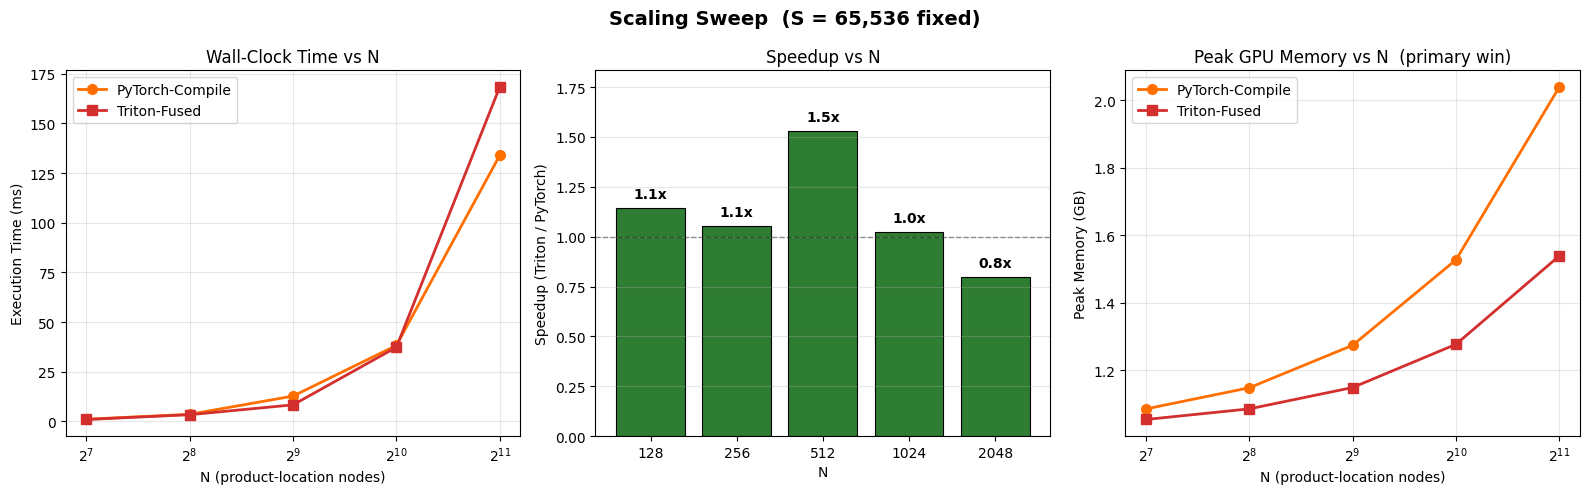
\includegraphics[width=\textwidth]{report_figures/scaling_sweep.png}
\caption{\emph{Left:} Execution time vs $N$. \emph{Centre:} Speedup ratio (1.0 baseline shown). \emph{Right:} Peak GPU memory---Triton consistently lower. The computation speedup is greatest at moderate $N$ (1.5$\times$ at $N{=}512$); at large $N$ the matmul dominates and both backends converge. Memory savings grow monotonically with $N$.}
\label{fig:scaling}
\end{figure}

The key finding is that \textbf{memory savings grow with problem scale} as the $\mathbf{D}$ matrix becomes a larger fraction of total memory, while computation speedup is most pronounced at moderate $N$ where element-wise fusion (profit logic) constitutes a larger fraction of total work. At large $N$, the $O(N^2 S)$ matmul dominates wall time and both backends generate efficient Triton code for it.

\section{Extension Results}\label{sec:ext-results}

All four extensions were benchmarked on the same T4 GPU with $N{=}2048$, $S{=}131{,}072$. \Cref{tab:ext-results} summarises performance.

\begin{table}[H]
\centering\small
\caption{Extension benchmark results ($N{=}2048$, $S{=}131{,}072$, T4 GPU).}
\label{tab:ext-results}
\begin{tabular}{@{} l r r r r r @{}}
    \toprule
    \textbf{Extension} & \textbf{PT (ms)} & \textbf{TR (ms)} & \textbf{Speedup} & \textbf{TR Mem} & \textbf{PT Mem} \\
    \midrule
    Grid Search ($K{=}64$)   & 562.0 & 416.7 & 1.3$\times$ & 1.025\,GB & 3.024\,GB \\
    CVaR ($\alpha{=}0.05$)   & 633.7 & 383.6 & 1.7$\times$ & 1.028\,GB & 10.0\,GB\phantom{0} \\
    Budget (bisection)       & ---   & 18{,}123 & ---      & 1.028\,GB & --- \\
    Substitution             & 304.9 & 755.5 & 0.4$\times$ & 2.026\,GB & 2.026\,GB \\
    \bottomrule
\end{tabular}
\end{table}

\subsection{Grid Search Q* Analysis}

The Triton grid search kernel achieves a \textbf{1.3$\times$ speedup} and \textbf{66\% memory reduction} (3.024\,GB $\to$ 1.025\,GB) by evaluating expected profit at $K{=}64$ order quantities in a single fused pass. The kernel computes the matmul once and loops over $K$ Q-values entirely in SRAM.

\begin{figure}[H]
\centering
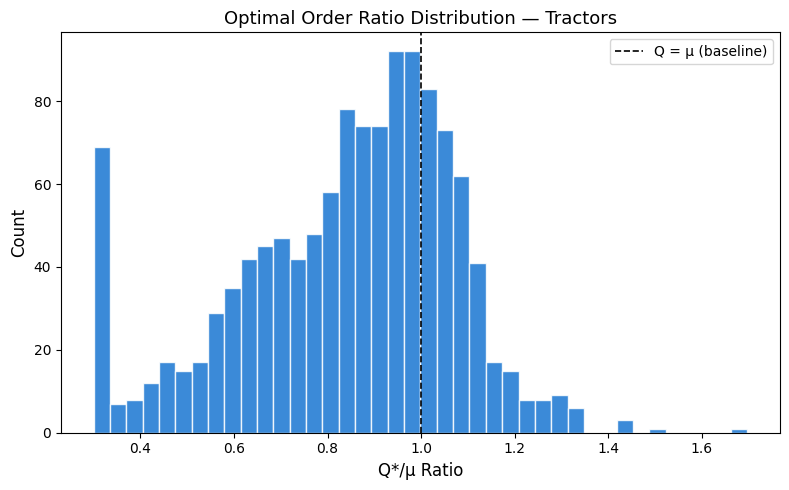
\includegraphics[width=0.48\textwidth]{report_figures/gs_qstar_ratio_tractors.png}\hfill
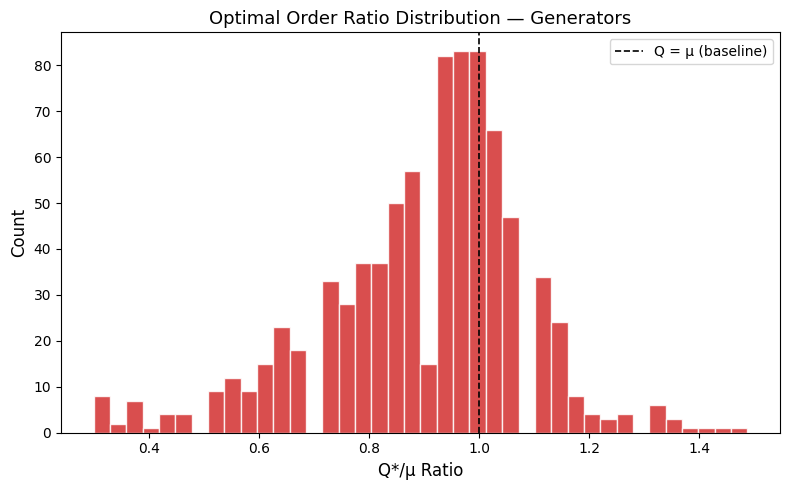
\includegraphics[width=0.48\textwidth]{report_figures/gs_qstar_ratio_generators.png}
\caption{Optimal order ratio $Q^*/\mu$ distribution. Mean $Q^*/\mu = 0.854$: 78\% of products should order \emph{less} than mean demand (newsvendor critical ratio effect). Tractors: mean 0.825; Generators: mean 0.899.}
\label{fig:gs-ratio}
\end{figure}

\begin{figure}[H]
\centering
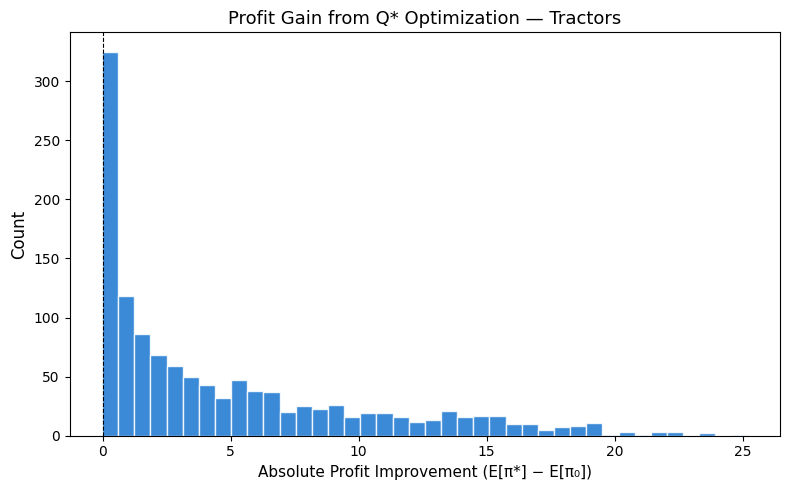
\includegraphics[width=0.48\textwidth]{report_figures/gs_profit_improvement_tractors.png}\hfill
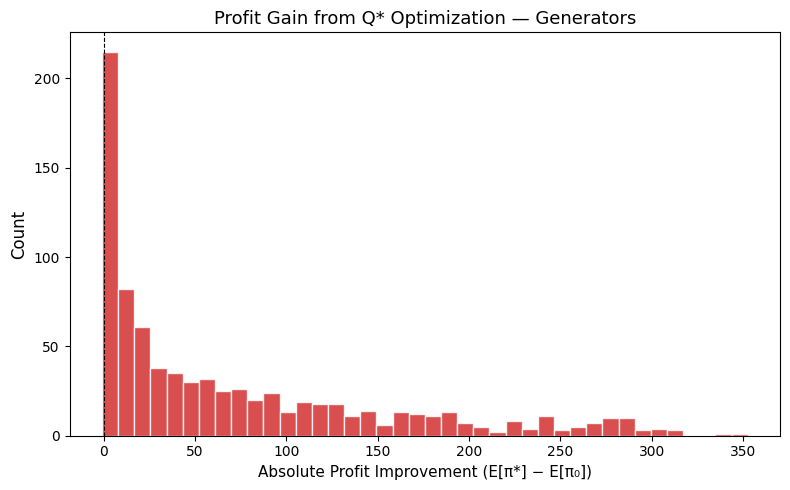
\includegraphics[width=0.48\textwidth]{report_figures/gs_profit_improvement_generators.png}
\caption{Absolute profit improvement per product from Q* optimisation. The right-skewed distribution shows that a minority of products benefit substantially from the optimal order quantity.}
\label{fig:gs-improvement}
\end{figure}

\begin{figure}[H]
\centering
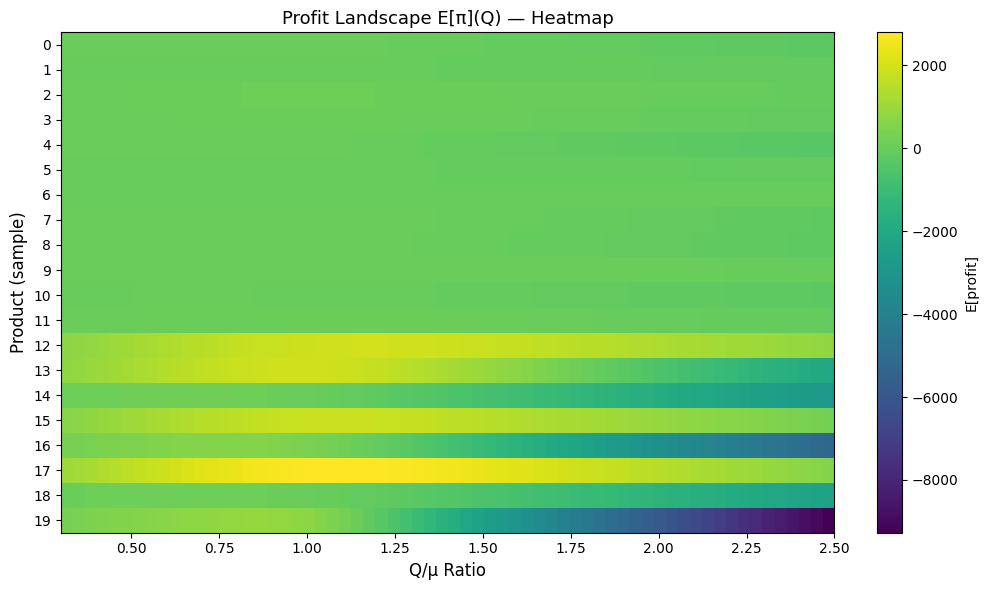
\includegraphics[width=0.55\textwidth]{report_figures/gs_profit_landscape_heatmap.png}
\caption{Profit landscape $\mathbb{E}[\pi](Q)$ heatmap for 20 sample products across the $K{=}64$ grid. Each row shows how expected profit varies with order-to-demand ratio. Products 12--19 (generators) show steeper profit sensitivity.}
\label{fig:gs-landscape}
\end{figure}

The aggregate profit improvement is \textbf{+5.3\%} ($\sum \mathbb{E}[\pi^*] = 1{,}266{,}338$ vs $\sum \mathbb{E}[\pi_0] = 1{,}202{,}184$). Numerical agreement between PyTorch and Triton is within 0.006 (max absolute difference), confirming correctness.

\subsection{CVaR Risk Analysis}

The CVaR kernel achieves a \textbf{1.7$\times$ speedup} and remarkable \textbf{90\% memory reduction} (10.0\,GB $\to$ 1.028\,GB). PyTorch must materialise the full profit matrix $[N,S]$ plus sorting intermediates for \texttt{torch.quantile}; the Triton kernel computes both expected profit and a 256-bin per-product histogram in a single fused pass.

\begin{figure}[H]
\centering
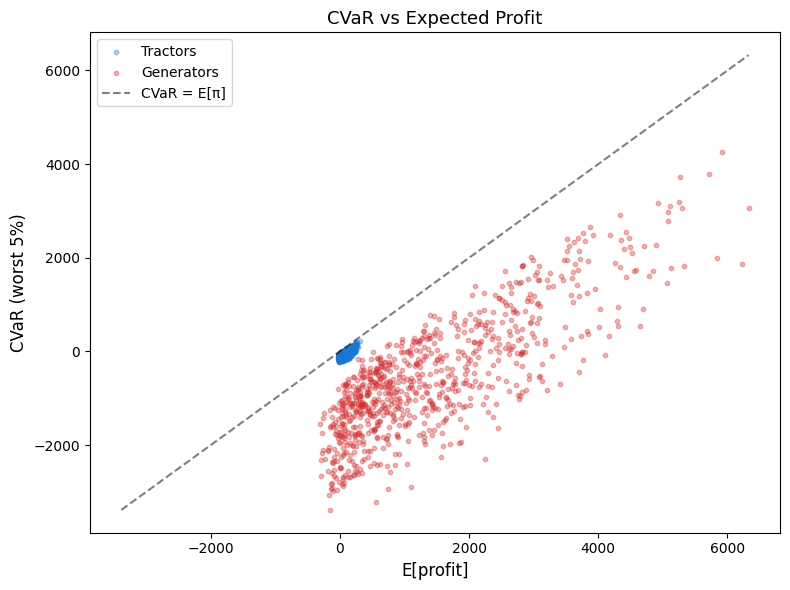
\includegraphics[width=0.55\textwidth]{report_figures/cvar_vs_eprofit_scatter.png}
\caption{CVaR vs Expected Profit. All points lie below the $y{=}x$ line (CVaR $\leq$ $\mathbb{E}[\pi]$), confirming coherence. Generators (red) exhibit wider dispersion---higher tail risk.}
\label{fig:cvar-scatter}
\end{figure}

\begin{figure}[H]
\centering
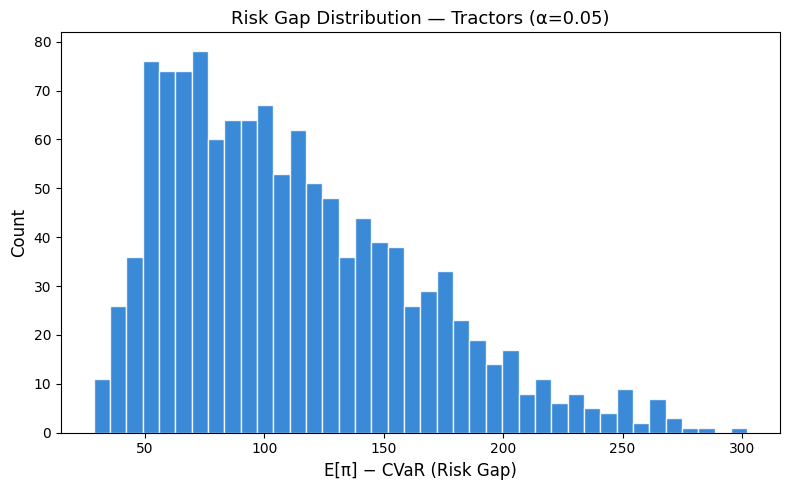
\includegraphics[width=0.48\textwidth]{report_figures/cvar_risk_gap_tractors.png}\hfill
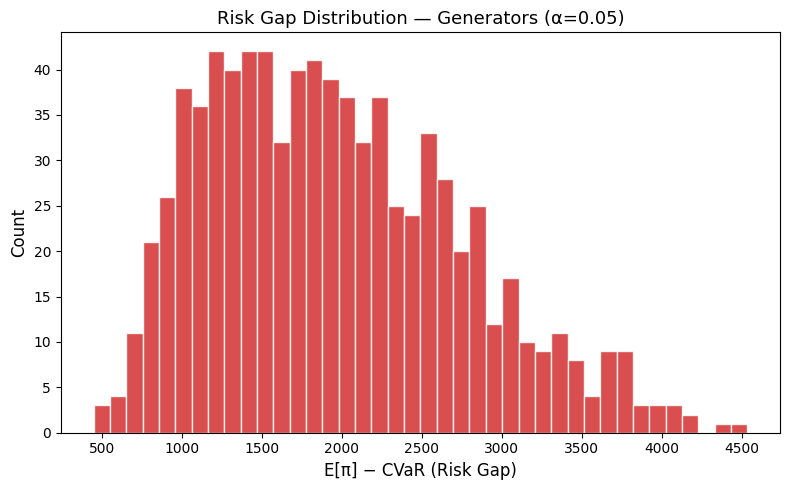
\includegraphics[width=0.48\textwidth]{report_figures/cvar_risk_gap_generators.png}
\caption{Risk gap ($\mathbb{E}[\pi] - \text{CVaR}$) distribution. Generators carry \textbf{17.5$\times$ more tail risk} on average (mean gap 1,955 vs 112), reflecting their higher demand variability and larger financial exposure.}
\label{fig:cvar-gap}
\end{figure}

VaR (5th percentile) ranges from $-2{,}776$ to $+4{,}653$ across products, with CVaR (expected worst-5\% profit) ranging from $-3{,}389$ to $+4{,}251$. The sanity check $\text{CVaR}_\alpha \leq \mathbb{E}[\pi]$ passes for all 2,048 products.

\subsection{Budget-Constrained Optimisation}

The Lagrangian bisection converges in \textbf{13 iterations} to $\lambda^* = 0.1575$, satisfying the budget $B = 2{,}116{,}484$ (70\% of unconstrained cost) with total procurement cost 2{,}116{,}461---within 0.001\% of the target. Total wall time is 18.1\,s (13 iterations $\times$ grid search kernel per iteration).

\begin{figure}[H]
\centering
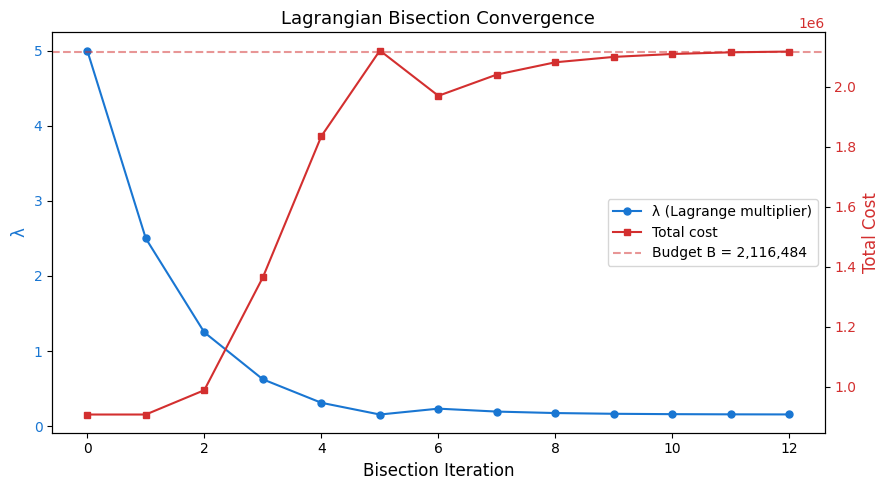
\includegraphics[width=0.55\textwidth]{report_figures/budget_bisection_convergence.png}
\caption{Lagrangian bisection convergence. The multiplier $\lambda$ (blue) decreases while total cost (red) rises to meet the budget constraint (dashed).}
\label{fig:budget-convergence}
\end{figure}

\begin{figure}[H]
\centering
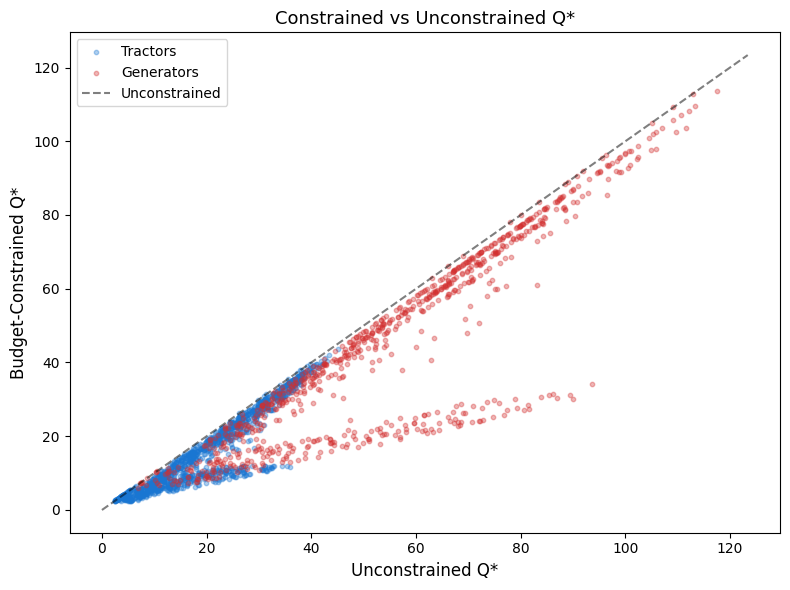
\includegraphics[width=0.48\textwidth]{report_figures/budget_constrained_vs_unconstrained.png}\hfill
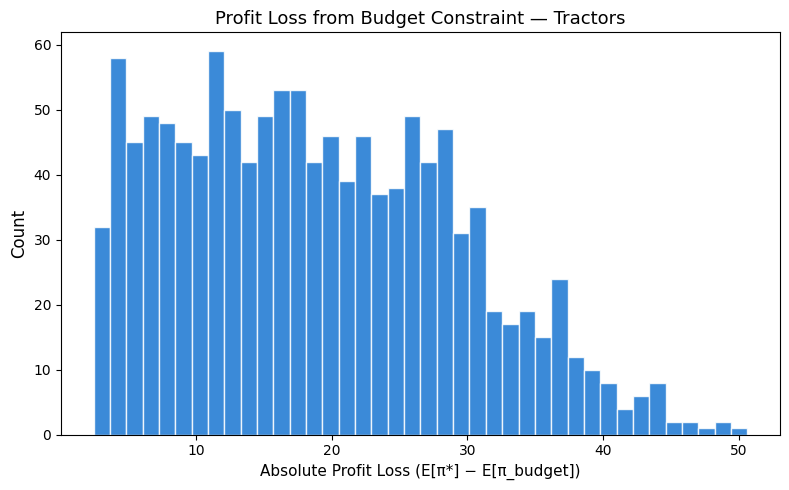
\includegraphics[width=0.48\textwidth]{report_figures/budget_profit_loss_tractors.png}
\caption{\emph{Left:} Constrained vs unconstrained $Q^*$ scatter---all points below the diagonal, confirming budget reduces order quantities. \emph{Right:} Absolute profit loss distribution for tractors.}
\label{fig:budget-analysis}
\end{figure}

The aggregate profit loss under the budget constraint is \textbf{30.7\%} ($\sum \mathbb{E}[\pi_\text{budget}] = 877{,}286$ vs $\sum \mathbb{E}[\pi^*] = 1{,}266{,}338$), with a mean $Q^*$ reduction of 21.9\%. This extension reuses the grid search kernel with no new Triton code---demonstrating modularity.

\subsection{Multi-Product Substitution}

Demand substitution increases aggregate profit by \textbf{+10.3\%} ($\sum \mathbb{E}[\pi_\text{sub}] = 1{,}325{,}760$ vs $\sum \mathbb{E}[\pi_0] = 1{,}202{,}184$), with an average of 3.27 units of redirected demand per product per scenario. All 2,048 products benefit from substitution.

\begin{figure}[H]
\centering
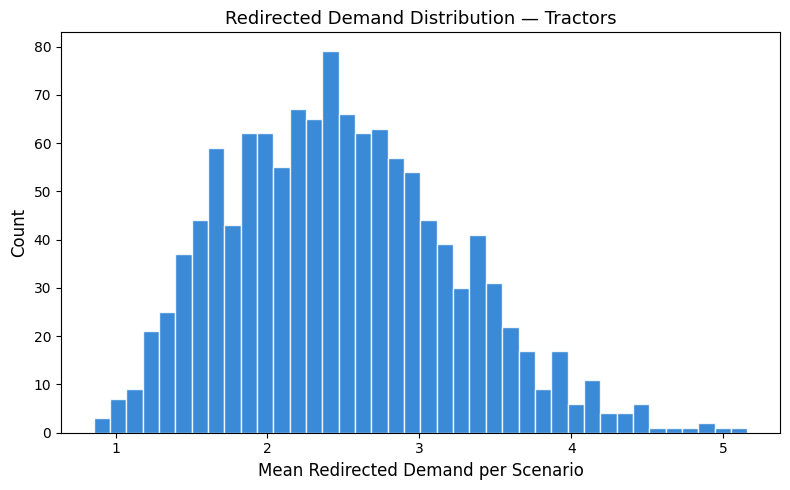
\includegraphics[width=0.48\textwidth]{report_figures/sub_redirected_demand_tractors.png}\hfill
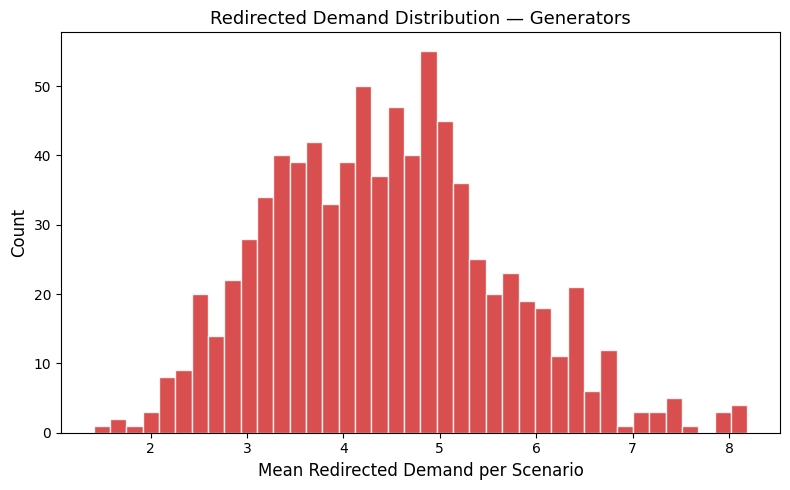
\includegraphics[width=0.48\textwidth]{report_figures/sub_redirected_demand_generators.png}
\caption{Redirected demand distribution. Generators redirect 1.8$\times$ more demand on average (4.44 vs 2.49 units), reflecting their higher stockout frequency.}
\label{fig:sub-demand}
\end{figure}

\begin{figure}[H]
\centering
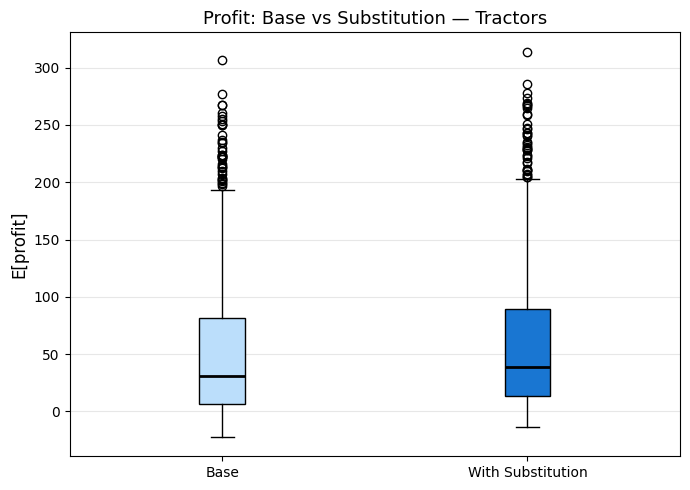
\includegraphics[width=0.48\textwidth]{report_figures/sub_boxplot_tractors.png}\hfill
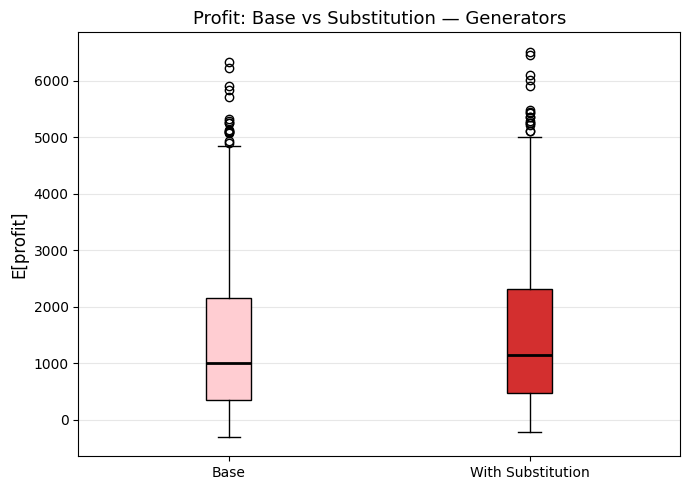
\includegraphics[width=0.48\textwidth]{report_figures/sub_boxplot_generators.png}
\caption{Profit comparison: base (Q=$\mu$) vs substitution. Both categories show upward median shift and tighter IQR, confirming that substitution provides both higher profit and reduced variance.}
\label{fig:sub-boxplot}
\end{figure}

The Triton two-pass kernel is \textbf{slower than PyTorch} (0.4$\times$) because the stockout matrix $[N,S]$ must be written to HBM between passes. This is a deliberate architectural choice and an important finding: SRAM fusion requires single-pass algorithms; multi-pass kernels with HBM intermediates do not benefit from tile-level fusion.

\section{Discussion}

The results reveal nuanced findings about the applicability of kernel fusion to Monte-Carlo inventory simulation.

\textbf{Memory efficiency as the primary contribution.} The 49.4\% peak memory reduction at full scale ($N{=}2048$, $S{=}131{,}072$) is the kernel's most consistent and impactful benefit. The intermediate $\mathbf{D}[N,S]$ matrix is a transient quantity---computed by the matmul, consumed once by the element-wise business logic, and immediately discarded. This producer-consumer pattern is the ideal candidate for kernel fusion, as recognised by Dao et al.~\citep{dao2022} for the attention score matrix in transformers. The 1.0\,GB memory saving is not merely a storage benefit; it enables larger problem instances on memory-constrained hardware and reduces the HBM bandwidth consumed by $\sim$75\%.

\textbf{Computation speedup depends on fusion fraction.} The base kernel's wall time at $N{=}2048$ is comparable to PyTorch-Compile because the $O(N^2 S)$ matmul dominates, and PyTorch Inductor itself generates efficient Triton code for this operation. However, the \emph{extension} kernels---Grid Search (1.3$\times$), CVaR (1.7$\times$)---demonstrate clear speedups because they fuse substantially more work per matmul tile (K grid-point evaluations, histogram binning). This pattern suggests that the benefit of manual kernel fusion scales with the ratio of fused element-wise work to matmul work.

\textbf{Extension memory scaling.} The CVaR extension achieves a striking 90\% memory reduction because PyTorch must materialise the entire profit matrix and sorting intermediates for \texttt{torch.quantile}, totalling $\sim$10\,GB. The Triton kernel's in-SRAM histogram avoids all of this. This demonstrates that the fusion advantage compounds for more complex per-scenario computations.

\textbf{Limits of fusion for multi-pass algorithms.} The substitution kernel's 0.4$\times$ speedup is an honest negative finding with important architectural implications. When the algorithm \emph{requires} writing an intermediate to HBM (stockout$[N,S]$ for cross-product dependency resolution), the second pass must perform a full HBM read, negating the fusion benefit. This result delineates the boundary of SRAM fusion: it is most effective for single-pass, row-independent computations.

\textbf{Scaling implications.} Memory savings grow with problem scale (\Cref{tab:scaling}). For enterprise-scale networks ($N > 10{,}000$), the $\mathbf{D}$ matrix would exceed 40\,GB at $S{=}131{,}072$---far beyond any single GPU's HBM capacity---making the fused approach not merely more efficient but the \emph{only viable single-GPU solution}.
